\documentclass[11pt, aspectratio=169, table]{beamer}
  % papersize={16cm,9cm},

\mode<presentation>{}

%%%%%%%%%%%%%%%%%%%%%%%%%%%%%%
% load packages
% add packages if needed

%\usepackage[T1]{fontenc}
\usepackage[utf8]{inputenc}
\usepackage{xcolor}
\usepackage[english]{babel}
\usepackage{amsmath,amsfonts,amssymb,amsthm}
\usepackage{color}
\usepackage[tracking=smallcaps, letterspace=-55]{microtype} % package for font spacing
\usepackage[outline]{contour}
%\usepackage[perpage]{footmisc}
\usepackage{transparent} % for setting opacity of pictures
\usepackage{pifont} % for checkmark (\ding{51}) and cross (\ding{55})
\usepackage{booktabs,array} % for tables
\usepackage{graphicx} % for figures
\usepackage{tikz}
\usepackage{pgfpages}
\usepackage{ulem}
\usepackage{dirtytalk}
\usepackage{multicol}
\usepackage{minted}

%\graphicspath{} % to set the path of figures

\usetikzlibrary{shapes.multipart,positioning,matrix,external,shadows}

\renewcommand{\thefootnote}{\fnsymbol{footnote}}
\renewcommand{\thempfootnote}{\fnsymbol{mpfootnote}}

%\setbeameroption{show notes on second screen=bottom}

%%%%%%%%%%%%%%%%%%%%%%%%%%%%%%
% Fill in the following information: AUTHOR, TITLE, DATE

\author[Saska Dönges]{Saska Dönges}
\title[Snabbare maskiner]{Hur kan jag göra \linebreak
datamaskiner snabbare?}
\subtitle{Baserat på verkliga händelser (högst 90\% fabrikation)\linebreak
Alernativt: Snabba data strukturer för medicin och bioinformatik\footnote{Med material stulet från Travis Gagies DCC 2023 inledningsanförande}}
\date{27.3.2023, NaNu2023}%{\today}
\institute{Avdelningen för dataveteskap, Helsingfors Universitet}

%%%%%%%%%%%%%%%%%%%%%%%%%%%%%%
% set beamer colors

\definecolor{hyblue}{RGB}{0,155,255}
\setbeamercolor{alerted text}{fg=hyblue}
\setbeamercolor{structure}{fg=hyblue}

\setbeamertemplate{itemize item}{\color{hyblue}}

%%%%%%%%%%%%%%%%%%%%%%%%%%%%%%
% set font (helvetica plays the role of Arial)
\usepackage{helvet}
\renewcommand{\familydefault}{\sfdefault}

%%%%%%%%%%%%%%%%%%%%%%%%%%%%%%
% set frametitle

\setbeamercolor{frametitle}{fg=black}%{fg=hyblue}
\setbeamerfont{frametitle}{series=\bfseries, shape=\scshape, size=\huge}
\setbeamertemplate{frametitle}[default][left,leftskip=3.5cm] % left shift of frame title
\addtobeamertemplate{frametitle}{\vspace{0.5cm}}{\vspace{1cm}} % spacing above and below frame title

%%%%%%%%%%%%%%%%%%%%%%%%%%%%%%
% set footline and headline
\beamertemplatenavigationsymbolsempty
\setbeamertemplate{headline}{ }
\setbeamertemplate{footline}{%
	 \usebeamercolor[fg]{page number in head/foot}%
	 \usebeamerfont{page number in head/foot}%
	\hspace{0.5cm}	
	
\includegraphics[width=2.5cm]{HY__LC05_txt__L_3L_B3____BW_cropped}
	\hfill
	\insertshorttitle\ /\ \insertshortauthor	\hfill
	\insertdate	\hspace{0.5cm}
	\insertframenumber\,/\,\inserttotalframenumber \hspace{0.5cm} \vskip2pt%
}

%%%%%%%%%%%%%%%%%%%%%%%%%%%%%%
% Other style settings
\useinnertheme{circles}

%%%%%%%%%%%%%%%%%%%%%%%%%%%%%%
% For video
\usepackage{media9}%
\newcommand{\includemovie}[3]{%
\includemedia[%
width=#1,height=#2,%
activate=onclick,%
deactivate=pageclose,%
addresource=#3,%
flashvars={%
src=#3 % same path as in addresource!
%&autoPlay=true % default: false; if =true, automatically starts playback after activation (see option ‘activation)’
&loop=true % if loop=true, media is played in a loop
&controlBarAutoHideTimeout=0 %  time span before auto-hide
}%
]{}{StrobeMediaPlayback.swf}%
}

%%%%%%%%%%%%%%%%%%%%%%%%%%%%%%
%%%%%%%%%%%%%%%%%%%%%%%%%%%%%%

\begin{document}

%% Title slide with HY picture
%{
%\usebackgroundtemplate{
%\setlength{\unitlength}{1cm}
%\begin{picture}(16,9)
%\transparent{0.33}
%\put(0.3,0.8){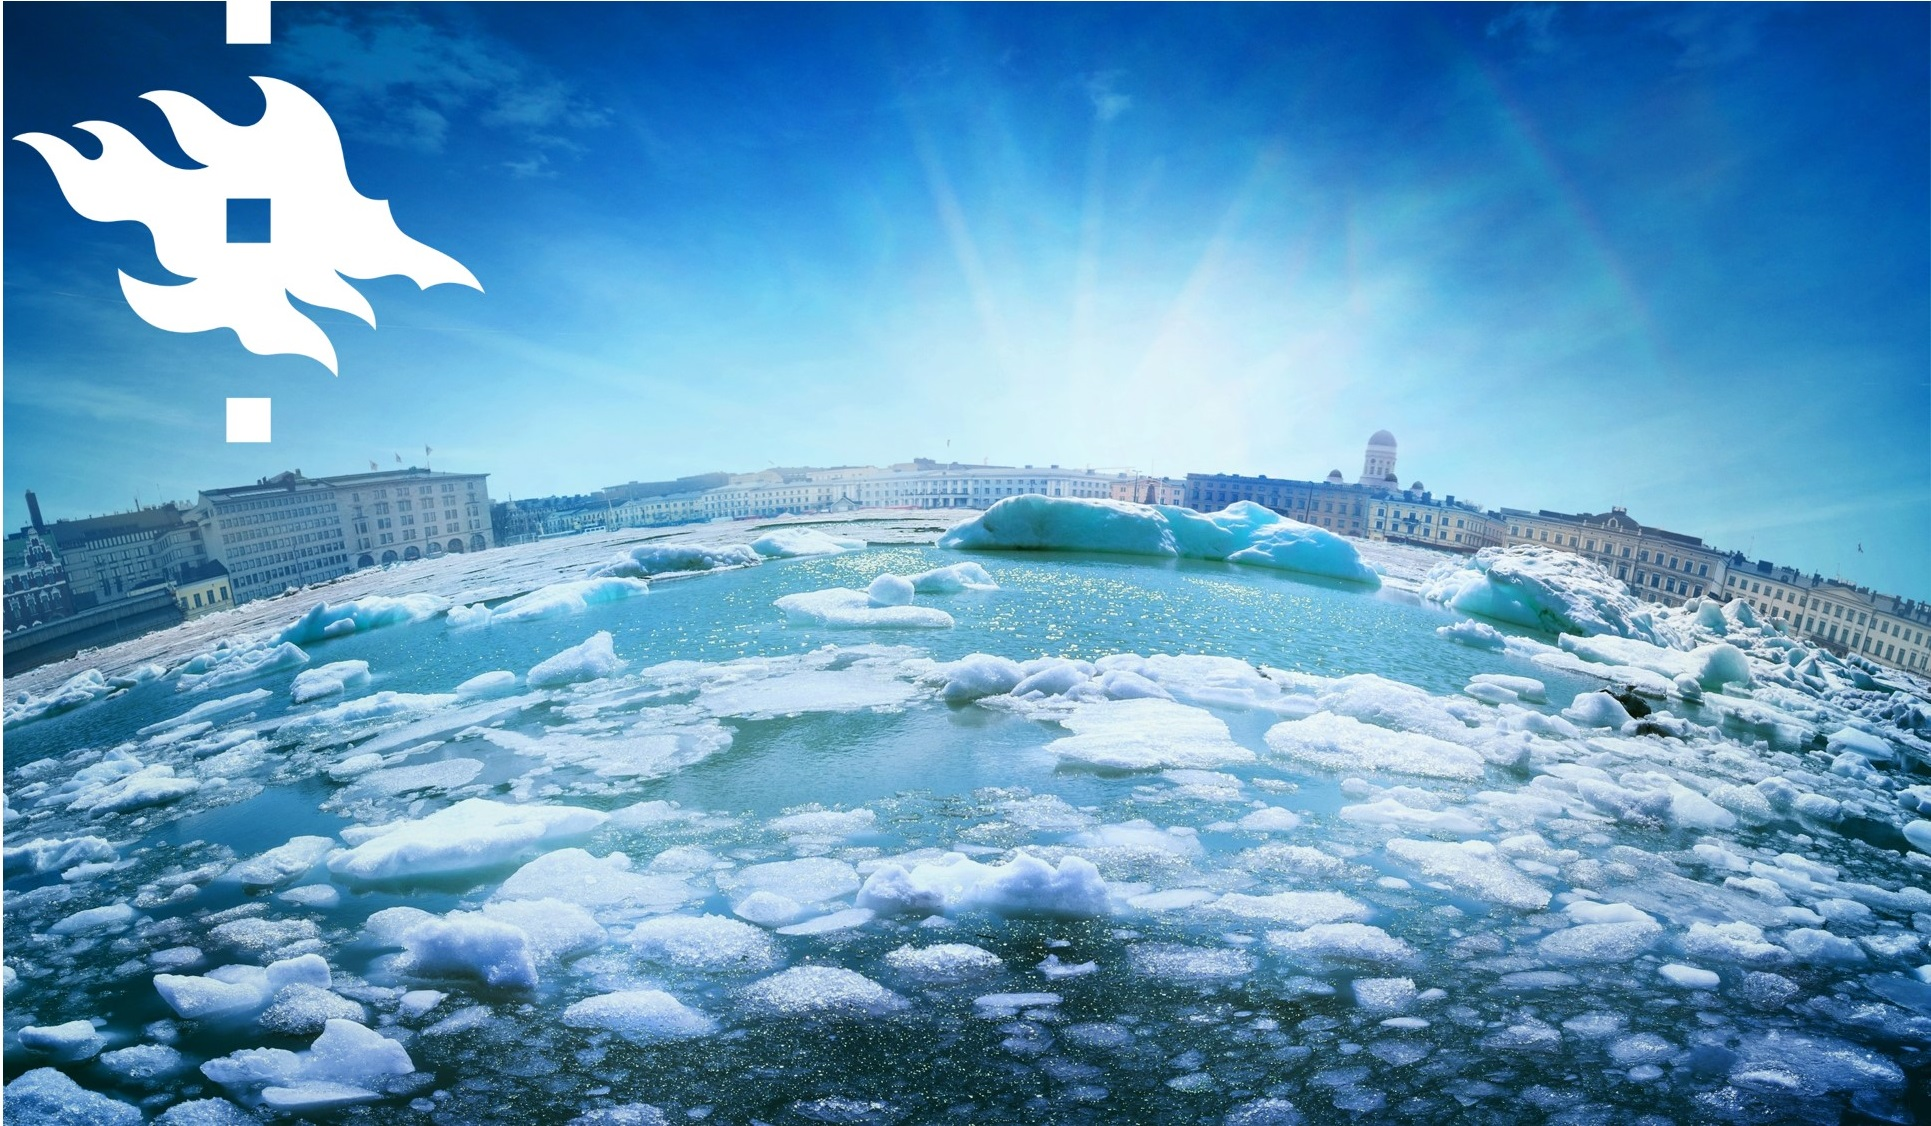
\includegraphics[width=15cm,height=7.8cm]{hy_brand_image_1_wide_background_hires_logo} }
%\end{picture}
%}
%\setbeamertemplate{headline}{ }%
%\begin{frame}{}
%\vspace{2.5cm}
%\begin{center}
%\huge
%{\bf \inserttitle } \\
%{\large \insertauthor}
%\end{center}
%\end{frame}
%}



% Title page without picture
{
\usebackgroundtemplate{
\setlength{\unitlength}{1cm}
\begin{picture}(16,9)
	\put(-0.1,5){ 
\includegraphics[width=4cm]{HY__LA01_Flame_____B3____BW} }
\end{picture}
\setlength{\unitlength}{1pt}
}
\setbeamertemplate{headline}{ }%
\begin{frame}[noframenumbering]{}
\vspace{2.5cm}
\begin{center}
\huge
\textcolor{hyblue}{ \bf
\inserttitle
} \\
{\large
{\bf\it \insertsubtitle} \linebreak
\insertauthor}
\end{center}
\end{frame}
}
%

%%%%%%%%%%%%%%%%%%%%%%%%%%%%%%
%% Main text

%% set HY Logo on the upper-left corner:
\usebackgroundtemplate{
\setlength{\unitlength}{1cm}
\begin{picture}(16,2.5)
\put(0.1,0){

\includegraphics[width=2.5cm]{HY__LA01_Flame_____B3____BW}\hfill
}
\end{picture}
\setlength{\unitlength}{1pt}
}
%%

%%%%%%%%%%%%%%%%%%%%%%%%%%%%%%
%% Modify text below

\begin{frame}{Agenda}
\setlength\parskip{\fill}
\tableofcontents
\end{frame}

\section{Vem är jag?}
\begin{frame}{Jag}
\setlength{\parskip}{\fill}
Doktorand i ``Compressed data structures'' gruppen, som är en del av supergruppen ``algorithmic bioinformatics''.

Borde disputera inom $\sim 1.5$ år.

Efter gymnasiet och milin studerade jag utomlands i några år tills jag burnouttade och flyttade tillbaka till Finland.

Jobbade några år ``inom industrin'' tills jag fick nog.

Startade på uni hösten 2015 $\to$ magister på våren 2021.
\end{frame}

\section{Berättelsen}
\begin{frame}{Berättelsen}
\setlength{\parskip}{\fill}
Jag återkommer till medicin, bioinformatik och mer detaljerad information om forskningsresultat om jag har tid.

Men först, en berättelse om min forsking, som kanske skulle kunna vara sann.
\end{frame}

\begin{frame}{Datamaskiner är snabba}
\setlength{\parskip}{\fill}
En modern dator kan göra miljontals meningsfulla beräkningar per sekund.

Men datorer är dumma. De gör \alert{exakt} vad som bes av dem. 

Även om det skulle kunna finnas bättre sätt att göra saker.

Gör en svår sak enklare för datorn $\Leftrightarrow$ Datorn kan beräkna saken snabbare.
\end{frame}

\begin{frame}{Multiplikation}
\setlength{\parskip}{\fill}
Det är (inte speciellt) svårt att beräkna $70 \cdot 300$.

Det är enklare att räkna $7 \cdot 3 \cdot 10 \cdot 100$. ``$21$ och tre nollor'' $= 21000$.

Skulle dethär vara något som vi skulle kunna hjälpa datorer med?

\pause
Nej. Tyvärr är datorer bra på att multiplicera, och bryr sig inte egentligen om vilka tal som används.

\pause
Men kanske division...
\end{frame}

\begin{frame}{Division}
\setlength{\parskip}{\fill}
Det är (inte speciellt) svårt att beräkna $1000 / 300$.

Det är enklare att ta $\frac{1000 / 100}{3}$. ``Ta bort $2$ nollor och dividera med $3$'' $ = 10 / 3 = 3\frac{1}{3}$.

Skulle dethär vara något som vi skulle kunna hjälpa datorer med?

\pause
Jo! Fast inte så som jag gjorde åvan.
\end{frame}

\begin{frame}{Division}
\setlength{\parskip}{\fill}
Det visar sig att datorer inte är speciellt bra på att dividera. Det skulle vara bättre att multiplicera i stället.

Så i stället för att göra $1000 / 300$ kan vi göra $1000 \cdot 0.0033333\ldots$.

Eller om vi arbetar med 32-bitars heltal kan vi göra $1000 \cdot 458129845 \gg 37$ I stället.

Altså vi sparar resultetet av $1000 \cdot 458129845$ som ett 64-bitars heltal och skiftar sedan resultatet till höger med $37$ bitar.
\end{frame}

\begin{frame}[fragile]{Division}
\setlength{\parskip}{\fill}
\begin{tabular}{r c}
 & \texttt{0000000000000000000000000000000000000000000000000010011100010000} \\
$/$ & \texttt{0000000000000000000000000000000000000000000000000000000100101100} \\
\hline
$=$ & \texttt{0000000000000000000000000000000000000000000000000000000000}{\em\texttt{100001}} \\
\\
 & \texttt{0000000000000000000000000000000000000000000000000010011100010000} \\
$\cdot$ & \texttt{0000000000000000000000000000000000011011010011101000000110110101} \\
\hline
$=$ & \texttt{000000000000000000000}{\em\texttt{100001}}\texttt{0101010101010101010101010111001010000}
\end{tabular}

Tyvärr gör moderna kompilatorer det här automatiskt. (Det var inte jag som räknade ut lösningen på förra sidan.)
\end{frame}

\begin{frame}{Nå men strängökning då?}
\setlength{\parskip}{\fill}
Strängsökning går ut på att hitta förekomster för en söksträng $P$ med längden $m$ ur en (ofta lång) text $T$ med längden $n$.

Alternativt bara ta reda på om $P$ förekommer i $T$, eller hur många gånger $P$ förekommer i $T$.
\end{frame}

\begin{frame}[fragile]{Naiv algoritm för strängsöking}
\setlength{\parskip}{\fill}
En så kallad ``brute-force'' algoritm:

\begin{minted}{python}
def str_cont(T, P):
    for i in range(len(T) - len(P)):
        for j in range(len(P)):
            if (T[i + j] != P[j]):
                break
        else:
            return True
\end{minted}
\end{frame}

\begin{frame}[fragile]{Vad gör algoritmen?}
\setlength{\parskip}{\fill}
Sökningen sker genom att jämföra varje position inom $T$ med $P$

\texttt{aaaaaaaaaaaaaaaaaaaaaaaaaaaaaaaaaaaaaaaaaaaaaaaaa}\linebreak
{\color{green}\texttt{aaaaa}}{\color{red}\texttt{b}}{\color{gray}\texttt{~b matchade inte så vi hoppar till nästa position.}}\linebreak
{\color{green}\texttt{~aaaaa}}{\color{red}\texttt{b}}{\color{gray}\texttt{~b matchade inte.}}\linebreak
{\color{green}\texttt{~~aaaaa}}{\color{red}\texttt{b}}{\color{gray}\texttt{~b matchade inte.}}\linebreak
{\color{green}\texttt{~~~aaaaa}}{\color{red}\texttt{b}}{\color{gray}\texttt{~b matchade inte.}}\linebreak
{\color{green}\texttt{~~~~aaaaa}}{\color{red}\texttt{b}}{\color{gray}\texttt{~b matchade inte.}}\linebreak

Sökningen tar i värsta fall ungefär $c \cdot n \cdot m$ sekunder (där $c$ är en liten konstant. $\sim 1 / 10000000$ i det här fallet.)
\end{frame}

\begin{frame}[fragile]{Hur snabb är ``brute force'' algoritmen?}
\setlength{\parskip}{\fill}
\begin{minted}{python}
T = "a" * 100000
P = "a" * 99 + "b"
\end{minted}

$T$ är hundratusen ``a''n och $P$ är 99 ``a'' med ett ``b'' på slutet.

\begin{minted}{python}
%%timeit
str_cont(T, P)

1.45 s ± 3.12 ms per loop (mean ± std. dev. of 7 runs, 1 loop each)
\end{minted}
\end{frame}

\begin{frame}{Vad kan vi göra i stället för ``brute-force''?}
\vspace{-0.5cm}
I exemplet märkte ni äventuellt att vi använder ``massor'' med resurser för att jämföra a bokstäver som alltid matchar.

Då b bokstaven inte matchar ``vet'' vi ju att om fem stycken a matchade innan så matchar åtminstone fyra stycken i nästa position.

Vi kan i hoppa över alla de gråa a bokstäverna som vi vet att kommer att matcha.

\texttt{aaaaaaaaaaaaaaaaaaaaaaaaaaaaaaaaaaaaaaaaaaaaaaaaa}\linebreak
{\color{green}\texttt{aaaaa}}{\color{red}\texttt{b}}{\color{gray}\texttt{~b matchade inte så vi hoppar till nästa position.}}\linebreak
{\color{gray}\texttt{~aaaa}}{\color{green}\texttt{a}}{\color{red}\texttt{b}}{\color{gray}\texttt{~b matchade inte.}}\linebreak
{\color{gray}\texttt{~~aaaa}}{\color{green}\texttt{a}}{\color{red}\texttt{b}}{\color{gray}\texttt{~b matchade inte.}}\linebreak
{\color{gray}\texttt{~~~aaaa}}{\color{green}\texttt{a}}{\color{red}\texttt{b}}{\color{gray}\texttt{~b matchade inte.}}\linebreak
{\color{gray}\texttt{~~~~aaaa}}{\color{green}\texttt{a}}{\color{red}\texttt{b}}{\color{gray}\texttt{~b matchade inte.}}\linebreak
\end{frame}

\begin{frame}[fragile]{Tyvärr(?) har smarta människor redan tidigare märkt detta.}
\setlength{\parskip}{\fill}
1970 hittade James Morris och Donald Knuth på en bättre lösning oberoende av varandra. År 1977 publicerade Knuth och Morris 
tilsammans med Vaughan Pratt ett papper där en effektiv version av vad som nu kallas för \alert{KMP algoritmen}.

Denna, eller någon nyare (och ännu bättre) lösning är redan för det mesta implementerad i standard bibliotek av programmeringsspråk. 

\begin{minted}{shell}
%%timeit
hittades = P in T

403 µs ± 1.86 µs per loop (mean ± std. dev. of 7 runs, 1000 loops each)
\end{minted}
\end{frame}

\begin{frame}{Men vad om vi känner till $T$ på förhand?}
\setlength{\parskip}{\fill}
Hur ofta får vi egentligen bara ett $T$ och $P$ ur det blå för att genomföra en sökning?

I en analog värld där $T$ skulle kunna vara en bok, skulle vi bläddra bak i boken 
och hoppas att där finns ett index där vi kan slå upp $P$.

Kan vi bygga ett index för $T$ så att vi för alla framtida sökningar snabbare kan 
ta reda på om $P$ förekommer i $T$?

\pause
Det är klart vi kan! Annars skulle berättelsen ha ett ganska snopet slut.
\end{frame}

\begin{frame}{Burrows-Wheeler!}
\begin{columns}[onlytextwidth,T]
\column{\dimexpr\linewidth-50mm-5mm}
\setlength{\parskip}{1em}

\alert{Burrows-Wheeler transformen} $B$ av $T$ är en permutation av $T$ där bokstaven i position $k$ inom $B$ är 
bokstaven före den $k$:nde slutdelen, då alla slutdelar av $T$ sorteras.

Lite jobbig definition. 

Om $T = $ ``abrakadabra '' så får vi

$B = $ ``ard kraaaabb''.
\column{50mm}
\vspace{-0.5cm}
\begin{tabular}{| c | l |}
\hline
B & slutdelarna \\
\hline
a & \\
r & a \\
d & abra \\
& abrakadabra \\
k & adabra \\
r & akadabra \\
a & bra \\
a & brakadabra \\
a & dabra \\
a & kadabra \\
b & ra \\
b & rakadabra \\
\hline
\end{tabular}
\end{columns}
\end{frame}

\begin{frame}{Vad gör vi med $B$?}
\setlength{\parskip}{\fill}
Det visar sig att $B$ ofta är lätt att komprimera. Till exempel genom att i stället för att spara ``aaaa'' bara spara $a^4$.

Då skulle vi kunna spara $B$ som $a^1r^1d^1\;^1k^1r^1a^4b^2$. Vilket kanske inte verkar så fint.

Men för praktiska data sparar detta massor med utrymme.
\end{frame}

\begin{frame}[fragile]{Men varför vill vi ens ha $B$}
\setlength{\parskip}{\fill}
Om vi har $B$ och vet hur många av vilka bokstäver som finns i $B$, kan vi mycket snabbt räkna ut om $P$ 
förekommer i $T$ för ett godtyckligt $P$. Vi kan även enkelt ta reda på hur många gånger $P$ förekommer i $T$.

Med ``normal'' strängsöking kan vi (långsamt) räkna hur många gånger ``Einstein`` förekommer 
i \texttt{einstein.en.txt}\footnote{\url{http://pizzachili.dcc.uchile.cl/repcorpus.html}} 

\begin{minted}{shell}
grep -o 'Einstein' einstein.en.txt | wc -l
2475825
real	0m1.035s
user	0m1.004s
sys	0m0.053s
\end{minted}
\end{frame}

\begin{frame}[fragile]{Hur snabba är index strukturer för strängsökning?}
Med ett \alert{Burrows-wheeler} index kan vi räkna förekomsterna aningen snabbare:

\begin{minted}{shell}
time ./counting_exp einstein.en
pattern   count    time
Einstein  2475825  34649
Mean query time: 34649ns
 with 0.018994 bits per symbol.

real    0m0.006s
user    0m0.000s
sys     0m0.006s
\end{minted}
\end{frame}

\begin{frame}{Ännu snabbare!?}
\setlength{\parskip}{\fill}
Men vad hände med att göra datorer snabbare?

Nu har jag bara beskrivit helt nya sätt att göra mer eller mindre samma sak?

Det visar sig att strukturen jag demonstrerade  är ``teoretiskt optimal'' för vad den är.

Den tar så lite rum som möjligt och räknar förekomsterna i högst $c\cdot m$ sekunder (för någon konstant $c$).
\end{frame}

\begin{frame}{Hur gör jag datorer snabbare?}
\setlength{\parskip}{\fill}
Den teoretiskt optimala lösningen är inte optimal för datorn. 
Datastrukturen är byggd på ett sätt som gör att datorn konstant måste söka saker från olika delar av 
minnet för att göra de krävda beräkningarna.

(Som att bläddra fram och tillbaka i en bok om en text, bilder och tabeller som har att göra med samma sak är på helt olika sidor.)

Vi har designat en ny version av samma data struktur som går att använda för att beräkna förekomsterna i $c\cdot b \cdot m$ sekunder, 
där $b$ kan vara till exempel 32. Om $c$ för vår struktur 32 gånger mindre än tidigare versioner, är vår datastruktur snabbare.
\end{frame}

\begin{frame}[fragile]{Hur snabb är den då?}
\begin{minted}{shell}
time ./count_matches -c einstein.en.runs einstein.en.patterns
looking for patterns from einstein.en.patterns in einstein.en.runs
Pattern   count    time
Einstein  2475825  8305
Mean query time: 8305 / 1 = 8305ns
 with 0.0235753 bits per symbol
real    0m0.003s
user    0m0.003s
sys     0m0.000s
\end{minted}

Det visar sig att $c$ tydligen blir över hundra gånger mindre.
\end{frame}

\begin{frame}{Jag får (hoppeligen) åka till Barcelåna!}
\setlength{\parskip}{\fill}
Vi har skrivit ett papper som jag hoppeligen får presentera i Juli.
\end{frame}

\section{Motivation}
\begin{frame}{DNA sekvensering}
\setlength{\parskip}{\fill}
Då en människas genom sekvenseras, görs det i allmänhet med hjälp av ett referensgenom.

En sekvenseringsmaskin läser in små snuttar av en ny människas dna.

Rätt plats för snuttarna söks genom att gämföra till referensen.

\begin{center}
\tt \begin{tabular}{r|ccccccc}
\sf referens & G & A & T & A & C & A & T\\
\hline
\sf snutt 1 & G & A & T & A\\
\sf snutt 2 &   & A & T & A & C\\
\sf snutt 3 &   &   &   & A & C & A & T
\end{tabular}
\end{center}
\end{frame}

\begin{frame}{DNA sekvensering}
\setlength{\parskip}{\fill}
Fungerar ofta ganska bra.

Men om den nya individen har små mutationer som inte kommer överens med referensen kan det uppstå problem.

\begin{center}
\tt \begin{tabular}{r|cccccccc}
\sf reference & G & A & T & T & A & C & A & T\\
\hline
\sf read 1    & G & A & T & - & A\\
\sf read 2    &   & \textcolor{gray}{A} & \textcolor{gray}{-} & \textcolor{gray}{T} & \textcolor{gray}{A} & \textcolor{gray}{G}\\
\sf read 3    &   &   &   &   & \textcolor{gray}{A} & \textcolor{gray}{G} & \textcolor{gray}{A} & \textcolor{gray}{T}\\
\hline
\sf output    & G & A & T & - & A & C & A & T
\end{tabular}
\end{center}

I problemfall fyller man bara i med referensgenomen.
\end{frame}

\begin{frame}{Referens bias}
\small
\begin{quotation}
To the scientists' puzzlement, however, the boy's sequence showed no sign of the mutation in the gene known to 
cause Baratela Scott, called XYLT1. Nor did the DNA of the next boy with the disorder, or the next. As they 
tried to compare the boys' DNA sequences to the reference genome, it was like trying to check a spelling in a 
Webster's from which a prankster had torn handfuls of pages. Many pieces of the boys’ genomes, called short reads,
``weren’t in the reference genome at all,'' \dots\ There was no way to check them for disease-causing misspellings.
\end{quotation}

\hfill --- Sharon Begley, {\it Stat News}, March 11th, 2019
\end{frame}

\begin{frame}{Referens bias}
\small
\begin{quotation}
This bias limits the kind of genetic variation that can be detected, leaving some patients without diagnoses and 
potentially without proper treatment. What is more, people who share less ancestry with the man from Buffalo will 
probably benefit less from the incoming era of precision medicine, which promises to tailor healthcare to individuals.

[O]ur understanding of diversity within populations of European descent is now so good that we can start to use it 
for precision medicine. But for other populations, ``We do not have the same kind of data \dots\ [This] is going to 
increase healthcare disparities above and beyond what they are today.'' \dots\ [A] huge new project is offering a 
different solution with the aim to represent global diversity: a human pangenome.
\end{quotation}

\hfill --- Ida Emilie Steinmark, {\it Guardian}, January 29th, 2023
\end{frame}

\begin{frame}{Referens bias}
\small
\begin{quotation}
[T]he project is not just about sequencing more diverse data. ``We need to come up with a better data structure to 
encode that information,'' \dots\ That data structure is called a genome graph. In contrast to the current reference, 
which is just a long string of letters, the genome graph shows variation between genomes as detours on an otherwise 
shared path. That will enable researchers and doctors to map short reads to the version of the path that best fits their sample.
\end{quotation}

\hfill --- Ida Emilie Steinmark, {\it Guardian}, January 29th, 2023
\end{frame}

\begin{frame}{Pangenom graf}
Flere referensgenom:
\begin{itemize}
\item {\tt GATTACAT}
\item {\tt AGATACAT}
\item {\tt GATACAT}
\item {\tt GATTAGAT}
\item {\tt GATTAGATA}
\end{itemize}

\vfill

Pangenom graf utgående från referenserna:
\begin{center}
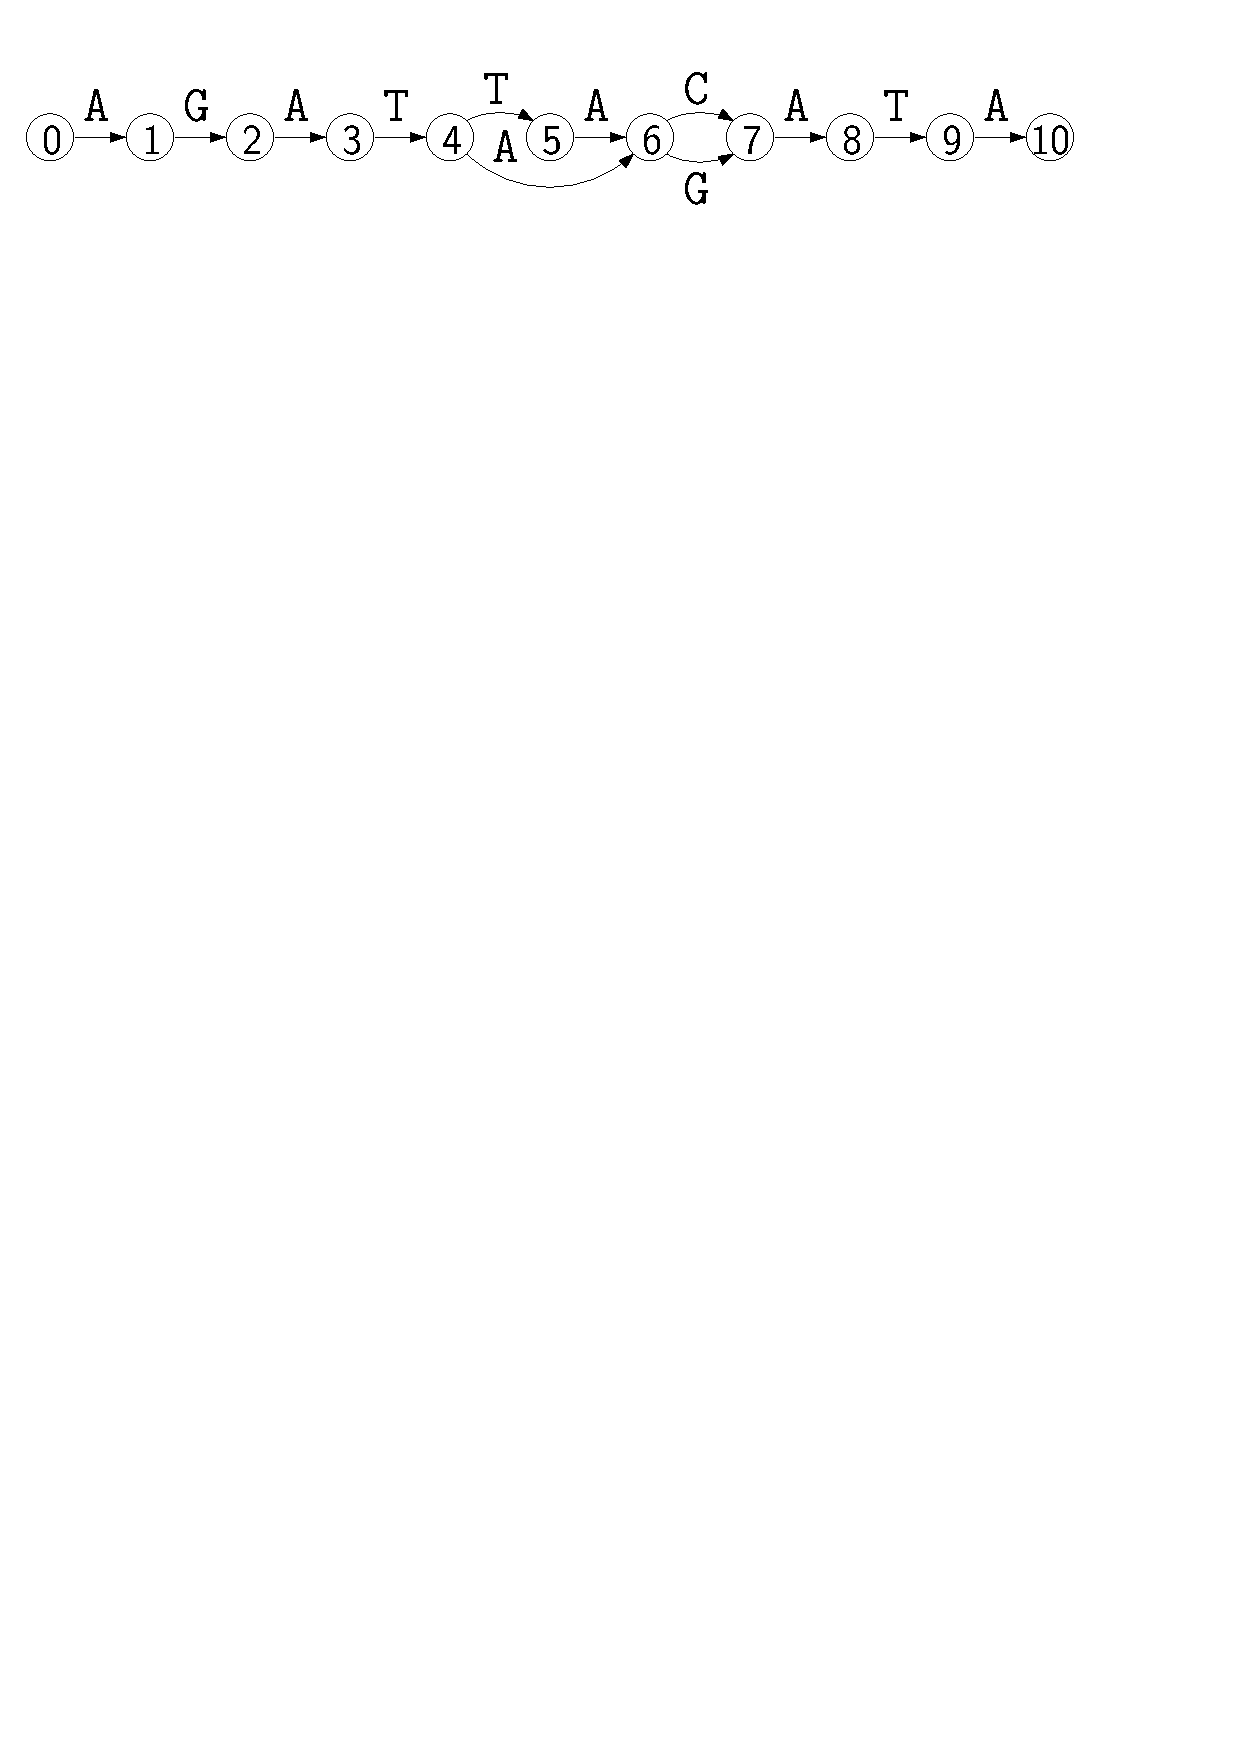
\includegraphics[width=.9\textwidth]{graph.pdf}
\end{center}
\end{frame}

\begin{frame}{Pangenom graf}
Referensgenom:
\begin{itemize}
\item {\tt GA3TTACAT}
\item {\tt AGATACAT}
\item {\tt GATACAT}
\item {\tt GATTAGAT}
\item {\tt GATTAGATA}
\end{itemize}

\vspace{-17ex}

\hspace{31ex} 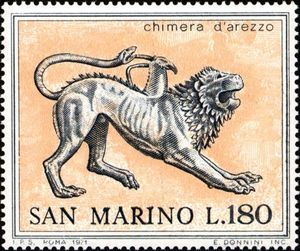
\includegraphics[width=.3\textwidth]{Chimera.jpg}

\vfill

Ser ut som om ``ATAG'' skulle vara en känd delsekvens
\begin{center}
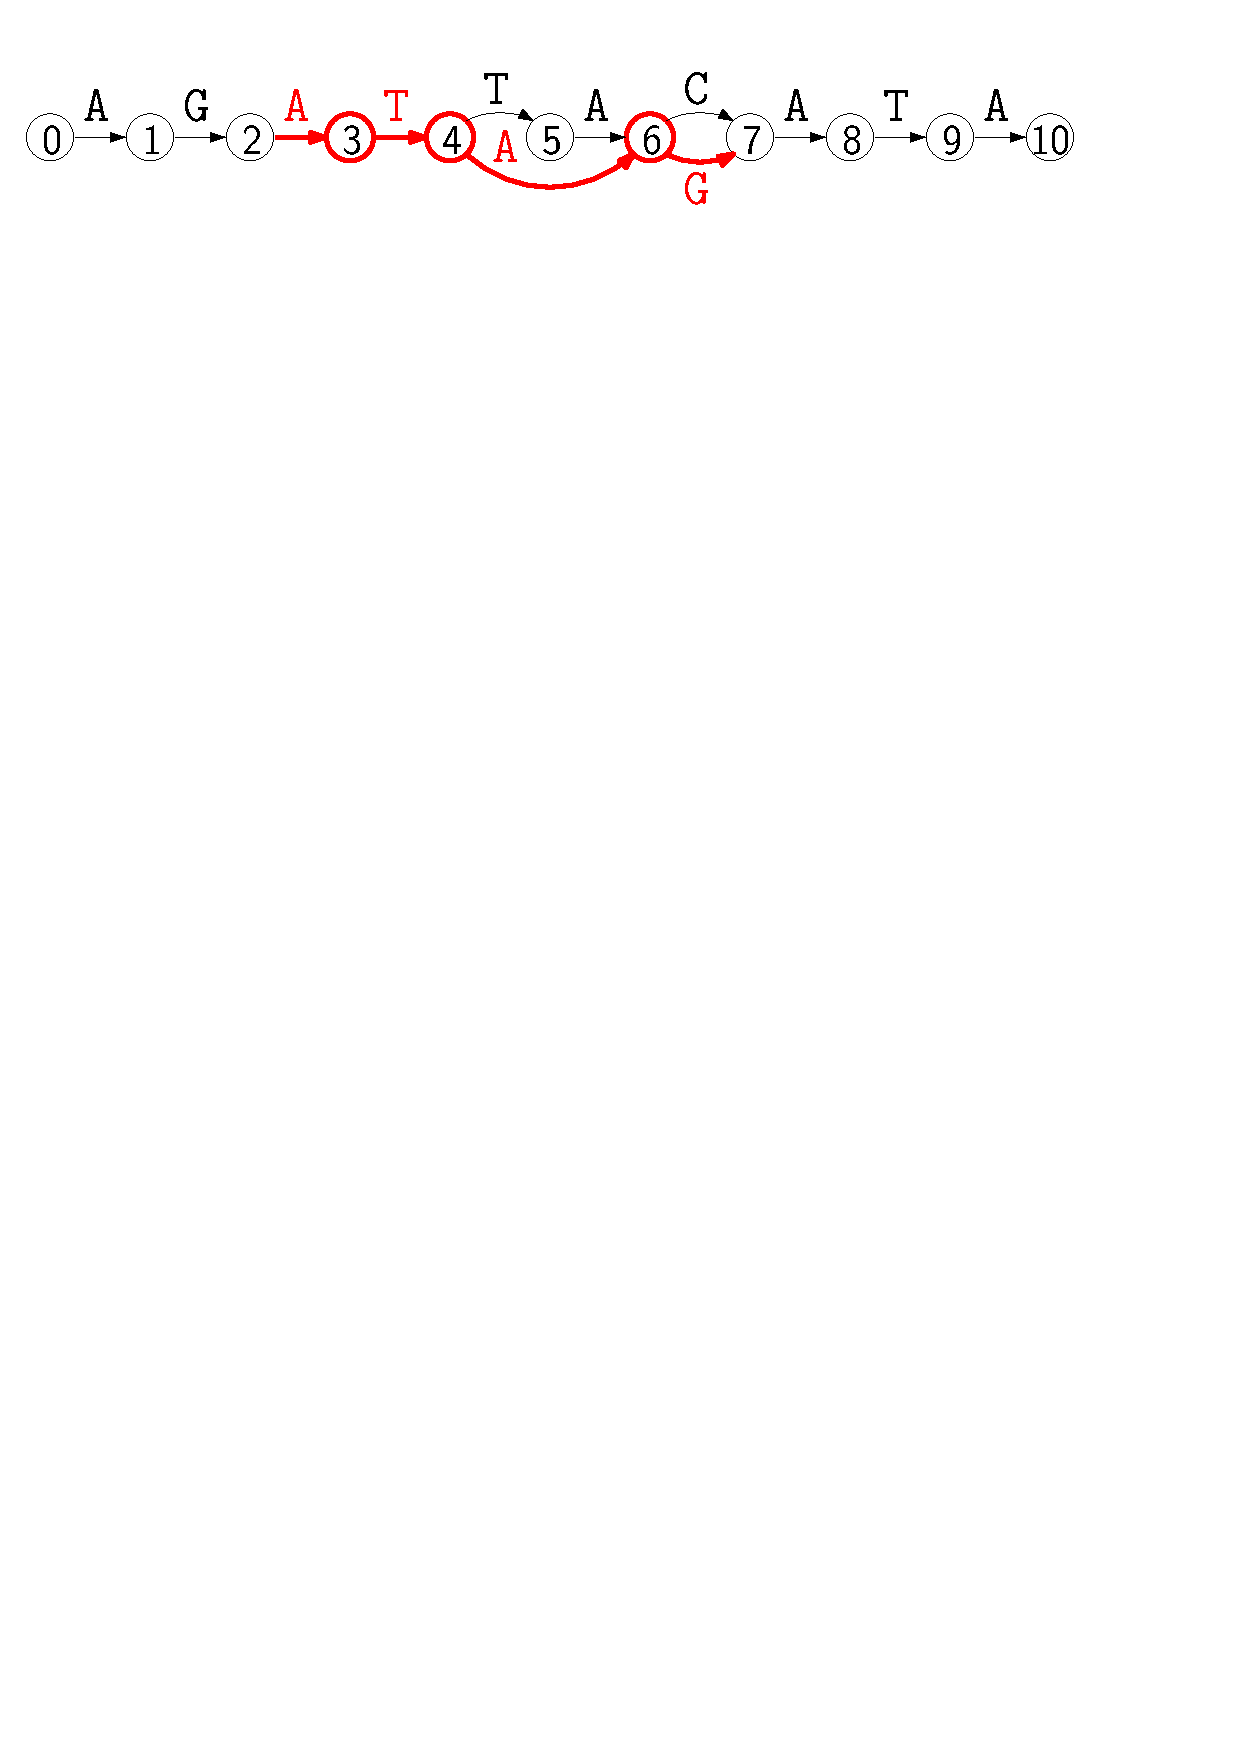
\includegraphics[width=.9\textwidth]{graph_ATAG.pdf}
\end{center}
\end{frame}

\begin{frame}{Pangenom graf}
Änne flere referensgenom:
\vspace{-0.3cm}\begin{multicols}{2}
\begin{itemize}
\item {\tt GATTACAT}
\item {\tt AGATACAT}
\item {\tt GATACAT}
\item {\tt GATTAGAT}
\item {\tt GATTAGATA}
\item {\tt CATTACAT}
\item {\tt GTTAGAT}
\item {\tt GATTCCATA}
\item {\tt GATTACAGA}
\item[]
\end{itemize}
\end{multicols}

\vspace{-0.3cm}Ännu svårare att veta vad som är riktigt och vad som inte är det
\begin{center}
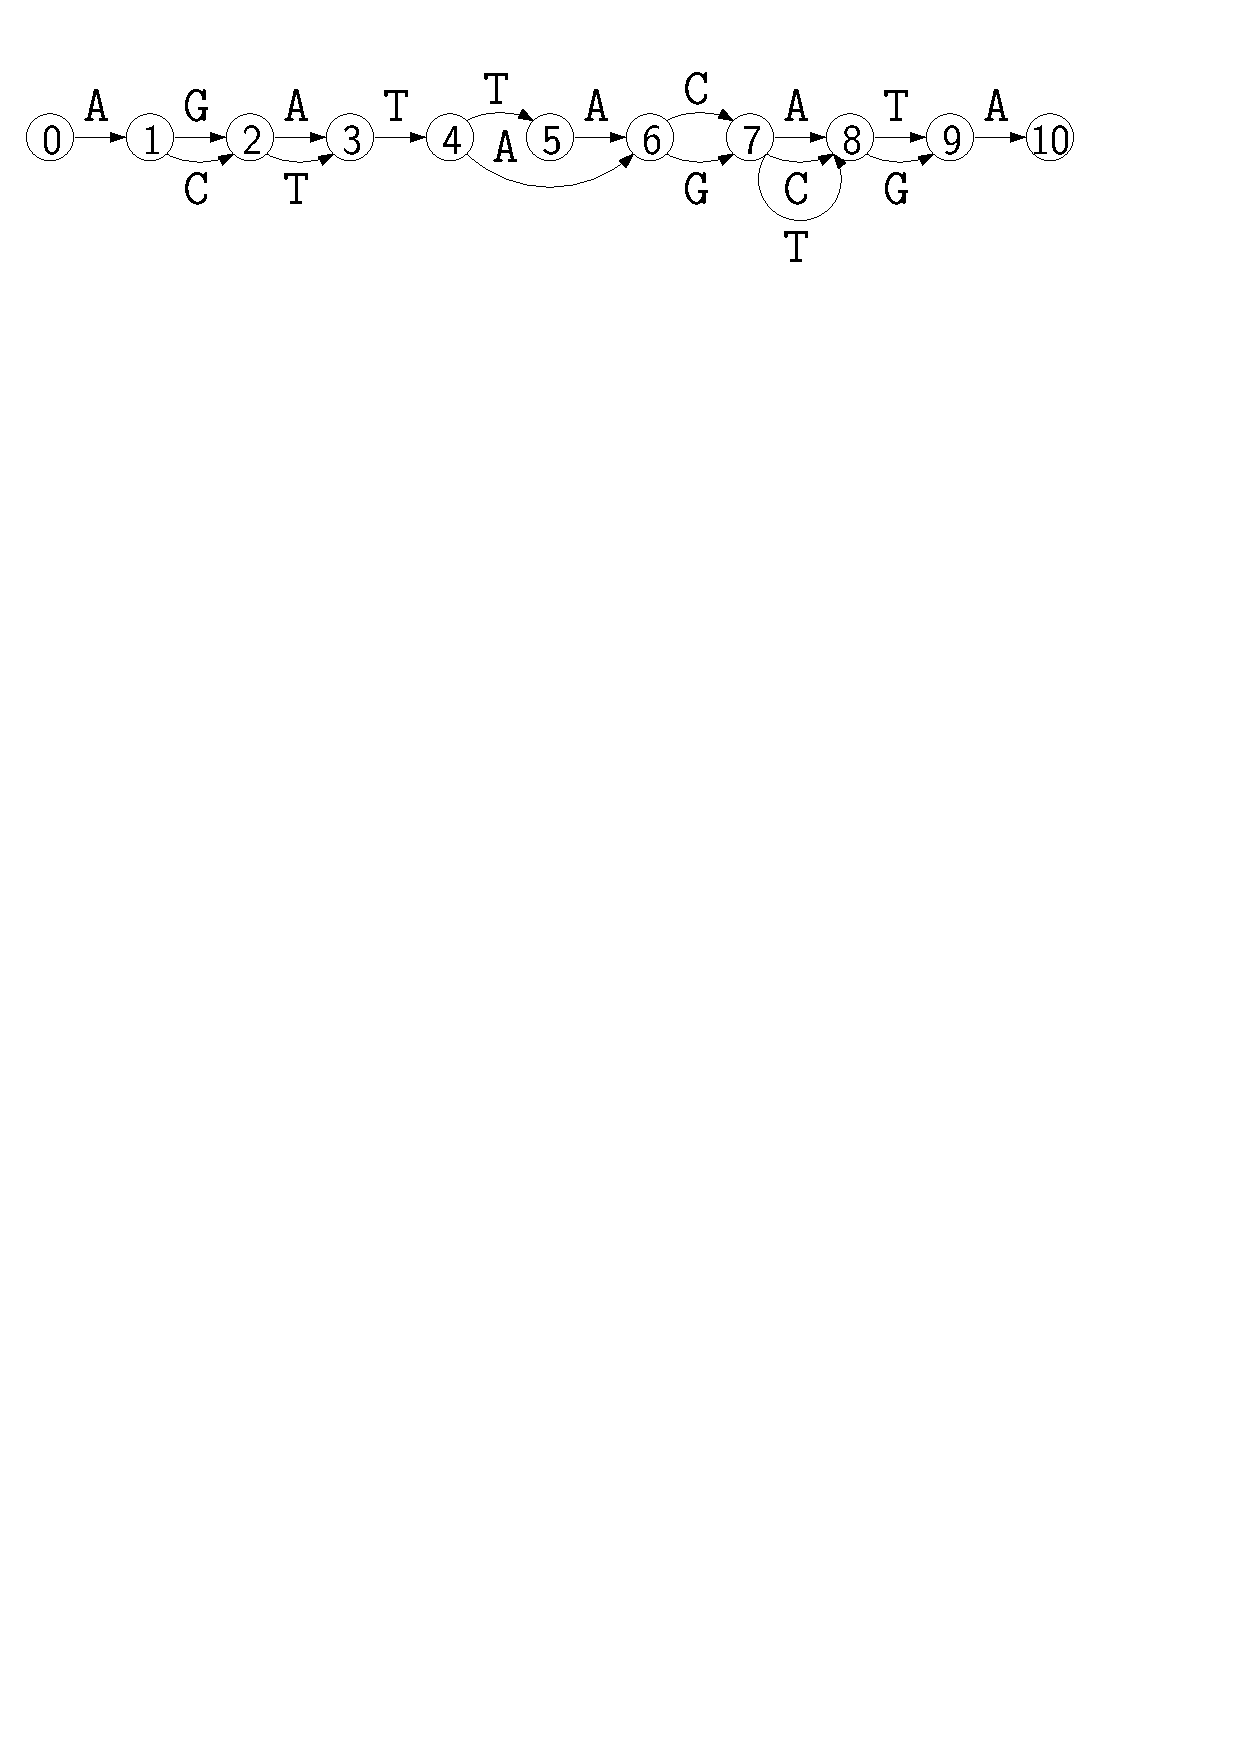
\includegraphics[width=.9\textwidth]{graph_fuzzy.pdf}
\end{center}
\end{frame}

\begin{frame}{Pangenom lösning}
\setlength{\parskip}{\fill}
Lösningen är att inte använda grafen för att hitta var en snutt hör till, utan att helt 
enkelt leta rätt på positionen genom att söka i alla referensgenom.

Problemet är att ett genom är hyfsat stort $\sim 700$ Megabit (lätt komprimerat).

Om vi vill söka i $100000$ referensgenom\footnote{\url{https://www.genomicsengland.co.uk/initiatives/100000-genomes-project}}, 
tar lätt komprimerade referenserna $70$ terabyte utrymme.

Ett effektivt komprimerat index kanske bara tar $\sim 1$ terabyte, vilket fortfarande är ganska mycket, 
men rymms i minnet av superdatorer.
\end{frame}

\section{Resultat}
\begin{frame}{Vår implementation är bra}
\begin{figure}
\centering
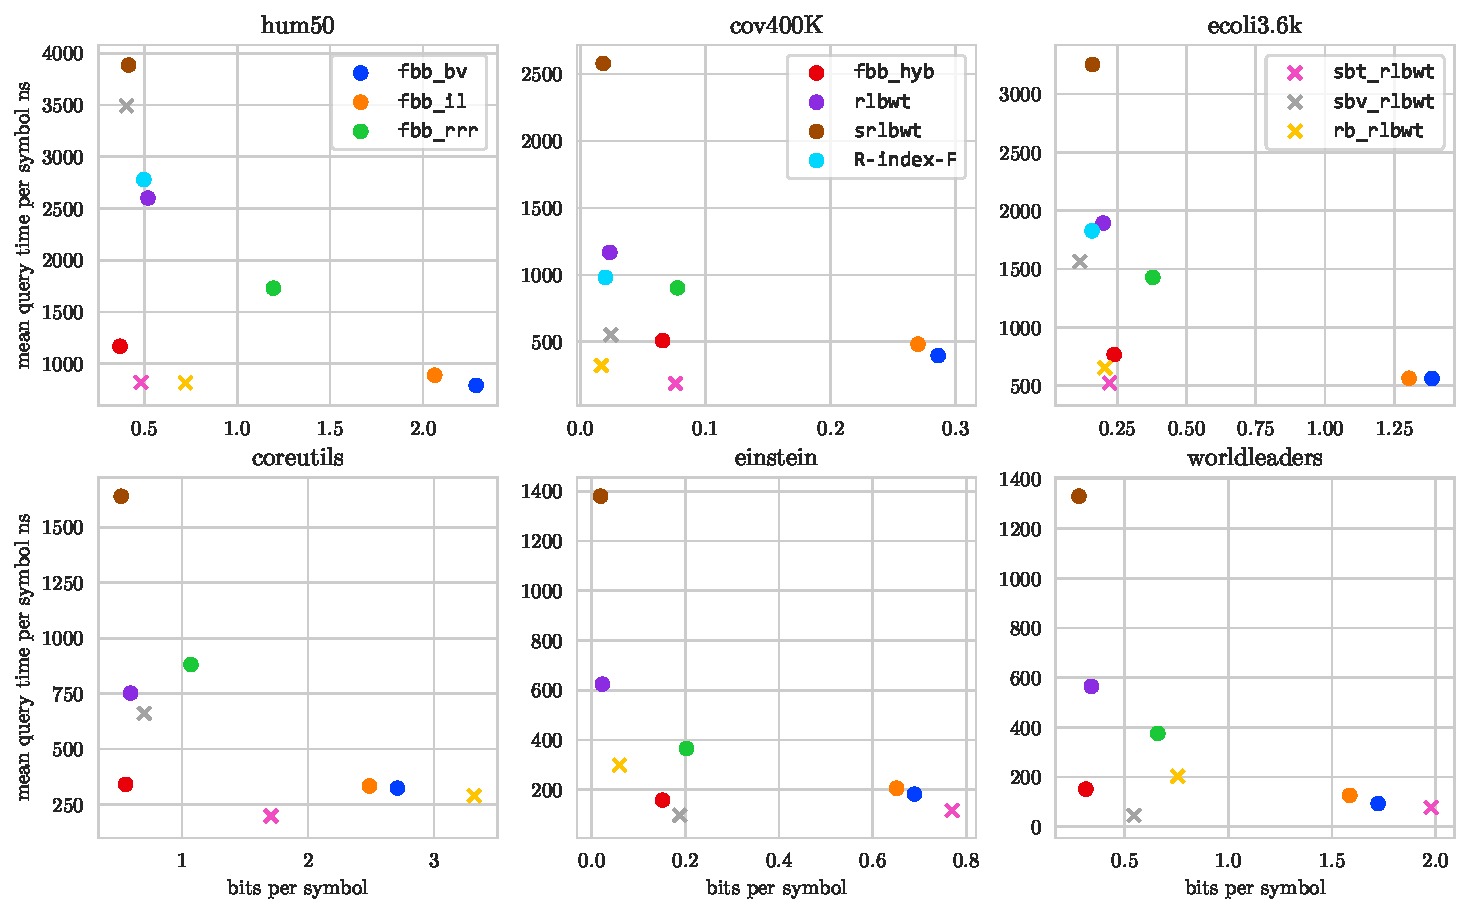
\includegraphics[trim={0 8cm 0 0},clip,width=\textwidth]{amd_pattern_count_30.pdf}
\end{figure}

Våra index indikeras med ``x''. De kräver mindre utrymme och är lika snabba som de snabbaste konkurrenterna.
\end{frame}

%{
%\usebackgroundtemplate{
%\transparent{0.3} % requires \usepackage{transparent} & compile twice
%\setlength{\unitlength}{1cm}
%\begin{picture}(16,9)
%\put(0.2,1){
%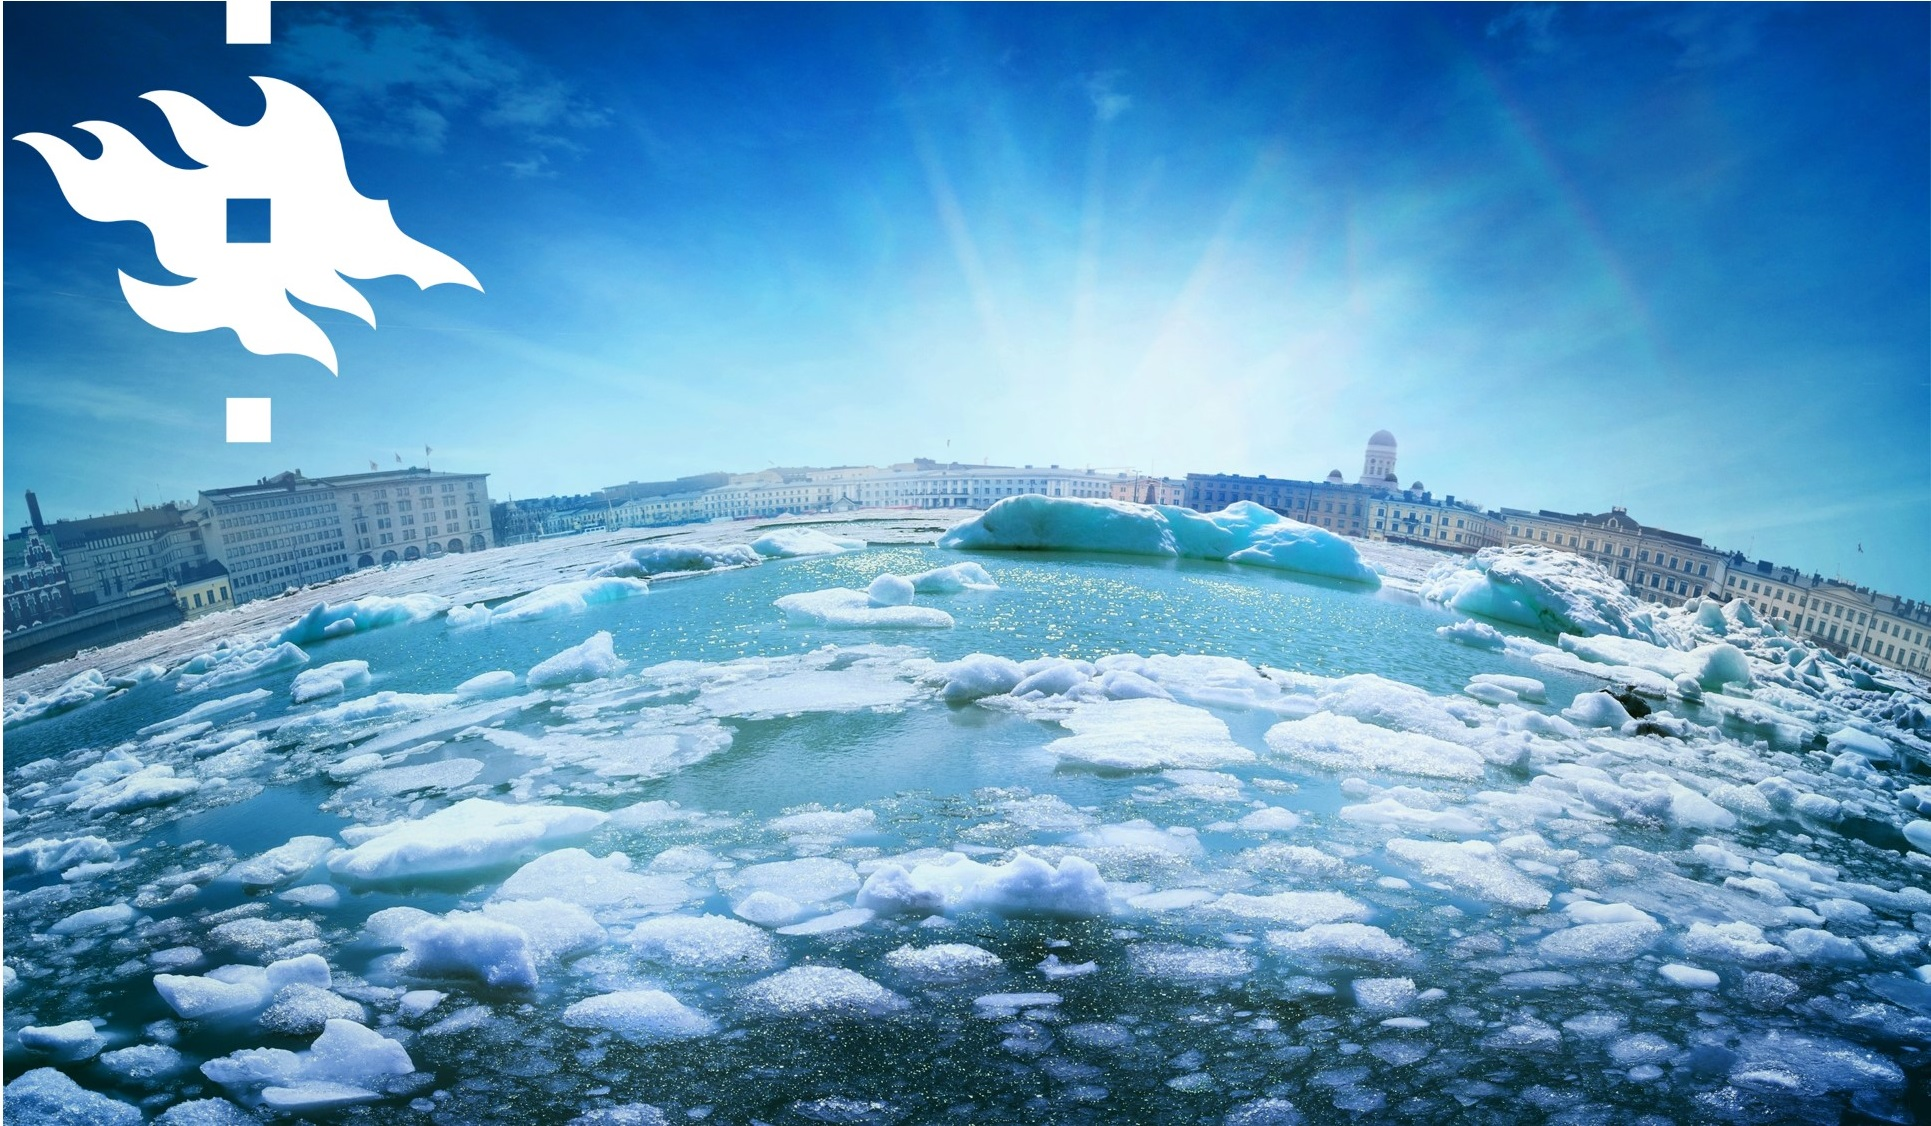
\includegraphics[width=15cm,height=7.5cm]{hy_brand_image_1_wide_background_hires_logo}
%}
%\end{picture}
%\setlength{\unitlength}{1pt}
%}
%
%\begin{frame}{\vspace{3cm}That's it}
%\begin{center}
%\vspace{-4cm}{\huge Questions?}
%\end{center}
%\end{frame}
%}

\end{document}





